% v2-acmsmall-sample.tex, dated March 6 2012
% This is a sample file for ACM small trim journals
%
% Compilation using 'acmsmall.cls' - version 1.3 (March 2012), Aptara Inc.
% (c) 2010 Association for Computing Machinery (ACM)
%
% Questions/Suggestions/Feedback should be addressed to => "acmtexsupport@aptaracorp.com".
% Users can also go through the FAQs available on the journal's submission webpage.
%
% Steps to compile: latex, bibtex, latex latex
%
% For tracking purposes => this is v1.3 - March 2012

\documentclass[prodmode,acmtosem]{acmsmall} % Aptara syntax

% Package to generate and customize Algorithm as per ACM style
\usepackage[ruled]{algorithm2e}
\usepackage{textcomp}
\usepackage{gensymb}
\usepackage[utf8]{inputenc}
\usepackage[table]{xcolor}
\usepackage{natbib}
\usepackage{subfigure}
\usepackage{tabularx}

\renewcommand{\algorithmcfname}{ALGORITHM}
\SetAlFnt{\small}
\SetAlCapFnt{\small}
\SetAlCapNameFnt{\small}
\SetAlCapHSkip{0pt}
\IncMargin{-\parindent}

% Metadata Information
% \acmVolume{9}
% \acmNumber{4}
% \acmArticle{39}
% \acmYear{2010}
% \acmMonth{3}

% Copyright
%\setcopyright{acmcopyright}
%\setcopyright{acmlicensed}
%\setcopyright{rightsretained}
%\setcopyright{usgov}
%\setcopyright{usgovmixed}
%\setcopyright{cagov}
%\setcopyright{cagovmixed}

% DOI
%\doi{0000001.0000001}

%ISSN
%\issn{1234-56789}

% Document starts
\begin{document}

% Page heads
\markboth{}{Dynamic obstacle mapping for the visually impaired using sensor fusion.}

% Title portion
\title{Dynamic obstacle mapping for the visually impaired using sensor fusion.}
\author{Johann Thor Kristthorsson
\affil{University College London}
Ifeanyi Ndu
\affil{University College London}
Veselin Pavlov
\affil{University College London}
Shuang Zhang
\affil{University College London}
}
% NOTE! Affiliations placed here should be for the institution where the
%       BULK of the research was done. If the author has gone to a new
%       institution, before publication, the (above) affiliation should NOT be changed.
%       The authors 'current' address may be given in the "Author's addresses:" block (below).
%       So for example, Mr. Abdelzaher, the bulk of the research was done at UIUC, and he is
%       currently affiliated with NASA.

\begin{abstract}
Abstract goes here
\end{abstract}


%
% The code below should be generated by the tool at
% http://dl.acm.org/ccs.cfm
% Please copy and paste the code instead of the example below. 
%
% \begin{CCSXML}
% <ccs2012>
%  <concept>
%   <concept_id>10010520.10010553.10010562</concept_id>
%   <concept_desc>Computer systems organization~Embedded systems</concept_desc>
%   <concept_significance>500</concept_significance>
%  </concept>
%  <concept>
%   <concept_id>10010520.10010575.10010755</concept_id>
%   <concept_desc>Computer systems organization~Redundancy</concept_desc>
%   <concept_significance>300</concept_significance>
%  </concept>
%  <concept>
%   <concept_id>10010520.10010553.10010554</concept_id>
%   <concept_desc>Computer systems organization~Robotics</concept_desc>
%   <concept_significance>100</concept_significance>
%  </concept>
%  <concept>
%   <concept_id>10003033.10003083.10003095</concept_id>
%   <concept_desc>Networks~Network reliability</concept_desc>
%   <concept_significance>100</concept_significance>
%  </concept>
% </ccs2012>  
% \end{CCSXML}

% \ccsdesc[500]{Computer systems organization~Embedded systems}
% \ccsdesc[300]{Computer systems organization~Redundancy}
% \ccsdesc{Computer systems organization~Robotics}
% \ccsdesc[100]{Networks~Network reliability}


\keywords{Sensor Fusion, Software Engineering,
Visually Impaired, Blind, Microsoft}

\acmformat{Johann Thor Kristthorsson, Ifeanyi Ndu, Veselin Pavlov and Shuang Zhang, 2016.}


% \begin{bottomstuff}
% This work was made in collaboration with Microsoft and the Guide Dogs association.
% \end{bottomstuff}

\maketitle

\section{Introduction}

Two million people are living with visual impairment in the UK, but despite that indoor environment are often not designed with this vast number of individuals in mind.\cite{NHSBlindStatistics} This situation leads creates stressful situations for the visually impaired and often forces them to depend on others to get around. Mobility canes and guide dogs work for this case but are limited in their use. The canes have restricted use to a person needing to navigate from place to place, and the guide dogs are not currently available to assist all visually impaired persons in the UK. Therefore, an easily available solution which can provide real-time assistance in an indoor environment for visually impaired people is highly needed. The Lighthouse team is working with Microsoft, which is both the sponsor and client of this project and who wanted the team to use wearable sensors to aid the visually impaired in this difficult situation.

To solve the problem mentioned above the team designed and built a platform which can process the data of the environment collected by sensors and give the user feedback about their surroundings, such as where they are and if there are obstacles nearby or not. There are two channels the application uses to notify the user of an obstacle.

The first is to poll the wearable sensors and immediately notify the user if they detect an obstacle the user is likely to collide with. The other is to query a server side platform for obstacles in the area. The sensor readings gathered in the first channel are sent to a server side platform for further processing where obstacles are identified and their location made available for all users of the platform. 

By cooperation of 8 MSc students in Lighthouse team, one data transfer API, one processing platform and an Android application were delivered. The API provide the communication between sensors and processing platform which generate the data collected with sensor fusion method and store result to the database. The Android application gives user feedback of surroundings by querying the database and showing the result on the map.
The Lighthouse platform reached the accuracy within one meter and controlled the latency to an acceptable range. The Lighthouse project not only solves the indoor dynamic obstacle mapping challenge but also makes it possible for visually impaired users to explore unfamiliar environments.


\section{Literature review} % TODO: Change to background
% TODO: Check if there is a difference in font size.
% TODO: use the 
% TODO: citet and citep
Obstacle detection is a large topic and has been popular in the last few years with the advent of autonomous vehicles and unmanned aerial vehicles.
The Defence Advanced Research Project Agency (DARPA) in the United States has held several competitions to push the research community towards this particular topic. The DARPA Grand Challenge in 2005 and the Urban Challenge in 2007 offered millions of dollars in prizes and sparked considerable interest within the research community~\cite{DARPAGrandChallenge2005,DARPAUrbanChallenge2007}.
\subsection{Obstacle detection}
In the specific case of obstacle detection as an assistive technology, there have been several papers exploring the topic. \citet{Cardin2007} developed a wearable system that uses an array of ultrasonic transducers to do sonar sensing of obstacles around a subject. The subject is notified of the obstacles through vibrotactile instruments sewn into clothing around the subject's torso. Experiments were conducted by blindfolding test subjects and having them navigate an environment filled with obstacles. The time it took the subjects to navigate was recorded, and the use of the system resulted in a 50\% reduction in navigation time after a short training time~\cite{Cardin2007}. The system developed by \citet{Shin2007} is similar to \citet{Cardin2007} but adds audible feedback through a headset~\cite{Shin2007}. These methods are entirely reactive, in that they sense and identify obstacles in space but do not record its position for possible future use. In addition to this, the evaluation of the detection accuracy is lacking. The studies do not describe their experimental setups accurately, and the data collection methods are never mentioned.
%These types of methods are common and widely explored both for the purposes of small robots and autonomous vehicles ~\cite{Kato2002}. 
%Shoval et al. have made attempts to fuse the work done in autonomous driving and robotics with the work in assistive technologies. They did this by mounting sonar sensing hardware on a robot that serves the same purpose as a guide dog. It has one axle and wheels that are powered. The robot is pushed by the subject via a handle, the robot can then detect and avoid obstacles and the subject notices the change in the robots movements through the handle ~\cite{Shoval2003}.
\subsection{Sensor Fusion}
Sensor fusion, or cooperative fusion, is a well-known term in the context of obstacle detection and navigation. This kind of technique combines the data from several sensors to get a more certain result than using sensors individually. \citet{Labayrade2005} describe algorithms and architectures that facilitate cooperative fusion of two different kinds of sensors, stereovision and LIDAR to detect obstacles in an autonomous driving scenario~\cite{Labayrade2005}. Cooperative fusion is used to detect barriers in the road in front of a vehicle and determine its distance with good accuracy. The use of sensor fusion decreased the rate of false negatives in the detection from 14.7\% and 5.2\% for LIDAR and stereovision respectively, down to 5.2\%. In addition the rate of false negatives went down from 4.5\% and 3.2\% respectively to 1.2\%. \citet{Cho2014} reached similar results showing an increase in the rate of true positives in obstacle detection from 83.2\% to 89.9\% by using fusion instead of using actual sensor values~\cite{Cho2014}. Contrary to the research found for the use cases for the visually impaired these papers provide a thorough explanation of the evaluation and data gathering performed and will prove useful in designing the evaluation strategy for this project. These methods have been developed specifically for use in the scenario of autonomous driving but are directly applicable to the scenario of detecting obstacles around a visually impaired pedestrian. Sensor fusion was introduced into the Windows 8 Operating system to provide stability to applications relying on clean and stabilised data. \citet{Gear2012} described a situation where engineers at Microsoft attempted to map a 3D virtual environment to a real environment in an app running on a tablet. First of all they tried emulate up and down movements in the virtual environment using an accelerometer. Almost immediately they encountered an issue when tilting the tablet and holding the tablet in a stationary position. Noise coming from the accelerometer alone caused jittery movements in the applications. To achieve a much more stable movement, the accelerometer readings was passed through a low-pass filter. The low-pass filter fulfilled its duty but simultaneously introduced a bottleneck into the app. Movement was significantly smoother but the motion in the app felt unresponsive and sluggish. The engineers also used a 6-axis compass which is a 3D accelerometer and 3D magnetometer to emulate left and right movements however it did not yield practicable result due to the instability of the 6-axis sensor. Finally the engineers hit a breakthrough with sensor fusion using the 3D accelerometer, 3D magnetometer and 3D gyroscope. Data collected from all 9-axis resulted in a smooth and fluid experience in the virtual app. Additionally the sensors complemented each other in terms of areas where they fell short~\cite{Gear2012}.

In light of research described in the literature reviewed the team will be able to reach the aims mentioned above of this project by developing a data collection platform that gathers data from many different cheap sensors. The sensor data will be used to identify obstacles, and the accuracy of the results will be increased by using sensor fusion.



% Add aims and goals
% What are we building now and what are it's aims


\subsection{Stakeholders and Project Context}
To identify and prioritise the goals and objectives of the SSE team first enumerated the stakeholders of the project and their desired outcomes. This would prove valuable to maintain a clear vision throughout the development process and to limit the risk of non-acceptance later on in the project.

\subsubsection{Microsoft}
Microsoft is both the sponsor and the client in this project, in addition to that Microsoft provides the team with access to domain experts and other resources. The primary outcome that Microsoft wants from the project is research into available assistive technologies based on obstacle detection and sensor fusion. The team is therefore responsible for conducting that research, enumerating the technologies available and developing a proof of concept prototype to illustrate the possibilities of a system using them.
Mr Jarnail Chudge is representing Microsoft and will be the team's client for the duration of the project.

\subsubsection{Visually Impaired People}
The Lighthouse team is working on solutions that can assist the blind or partly-sighted people in their daily life. The visually impaired people want to know where they are and what kind of objects are in their environment, especially in front of them, and they want to be informed particularly about the direction, the change in the environment and other persons. Given the fact that moving around independently is a desire of them, this project aims to improve the current situation when visually impaired people going into a unfamiliar indoor environment.
%\subsubsection{Academic}
%The academic administrators and supervisors of this project have a specific vision for how the team should apply their knowledge to the development process and client communication.The outcomes the academic stakeholders are interested in are having the team maintain rigorous documentation of the project, upholding the state of the art software engineering processes and maintaining good communication with the client throughout the process.

% \subsubsection{Team members}
% The team members have a different stake in the project since they want, not only, a good mark but also a rewarding learning experience.
% They want to see the project fulfilling the requirements of the other stakeholders while also getting a chance to tackle interesting and challenging problems that will widen their knowledge base in the field of Software Engineering.
% To ensure a passing mark for every member of the team, the SSE team aims to minimise the overall risk of the project and put in place contingencies in the event of possible non-acceptance of the project.

\subsection{High level goals}
%The team's initial contact with the client was a brainstorming session where he expressed the vision for the project. He expressed Microsoft's desire to have an end product which would feel natural to the user with very little work on the user's part regarding getting themselves familiar with the product. Then they raised the idea of using a sensor or combination of wearable sensors to achieve the ultimate goal. Ideas were then bounced around, and a subject area was found that was open for research and of value to our client.
%Microsoft Research has done some investigation into using sensor fusion and wanted to see how that technology could be utilised in aiding the visually impaired~\cite{Gear2012}.

%After the brainstorming session, the team met several times to brainstorm further and research possible applications around the sensor fusion concept and decided on a few possible project proposals.These were presented to the client, and he expressed interest in continuing with one of them.
For the final project proposal, our client agreed on a research area that will help the visually impaired navigate an indoor environment.
By using sensor fusion the team was to build a system that could collect data from various disparate sensors and identify the location of the user and obstacles in its environment.

The goal is to use cheap, off-the-shelf sensors and mitigate any error in the sensor readings by correlating different readings. This will help us reduce error and increase accuracy by using sensor fusion methods. The ones the team has selected to examine are the use of a Kalman filter, the central limit theorem and neural networks, in that order, to evaluate their applicability to the problem space. In order to identify the main goals of our client the team came up with scenarios and use cases, within the scope that was mentioned in section~\ref{sec:Prelim}, and presented them to the client. This was followed up by a discussion that leads to the identification of the following high level goals.


The main objective was to improve the experience of the visually impaired in a specific scenario. The scenario in question involved a visually impaired individual entering a space like a coffee shop and having to navigate around obstacles like tables and chairs.
This made obstacle detection a clear objective and secondary objectives relating to that were then further explored. The use of the obstacle detection in conjunction with detection of points of interest was discussed as a possible objective but was deemed less important by the client.
The use of Open Street Maps was discussed in this context as a database to work from with regards to gathering information on points of interest~\cite{OSM}.
Another secondary objective that came up on the topic of obstacle detection was the use of sensor fusion. Members of the Microsoft Research team had shown interest in the team evaluating sensor fusion techniques in the context of obstacle detection. This objective was deemed essential since it fit well with the rest of the project.

% Goal model diagram
% \begin{figure}
% \label{fig:GoalModel}
% \centering
% 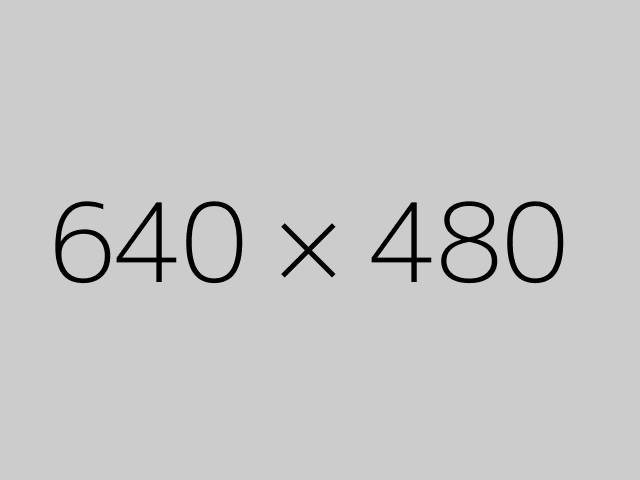
\includegraphics[width=\textwidth]{test640}
% \caption{An awesome goal model}
% \end{figure}

% TODO: Link to appendix with formal goal definitions

\subsection{Requirements}

Table \ref{table:1} shows a list of requirements our system will fulfill (please see section \ref{Appendix} for a full description of our requirement patterns).\\

\renewcommand{\arraystretch}{1.5}

\begin{center}
\begin{tabularx}{\textwidth}{| X | X |} 
 \hline
 \rowcolor{lightgray}
 \multicolumn{2}{|c|}{List of Requirements} \\ [0.5ex] 
 \hline\hline
 Identifying points of interest in the environment. &  Detecting obstacles \\
 \hline
 Feeding back mapping information &  Manually identifying obstacles in a space \\
 \hline
 Manually removing an obstacle from the map &  Providing navigation for a user to a point of interest \\ 
 \hline
 Voice interactions - listing &  Voice interactions - acceptance \\ 
 \hline
 Screen interactions - listing &  Screen interactions - acceptance \\ 
 \hline
 Classification of obstacles/Points Of Interest &  3D Directional Sound \\ 
 \hline
 Head Gestures &  IR and Ultrasound \\  
 \hline

 \hline
\end{tabularx}
\label{tab:requirements}
\end{center}

\section{System Architecture and Implementation}
\label{sec:architecture}
The architecture developed for this project is designed to be flexible and performant so that it allows for easy implementation of additional sensor inputs and can handle large volumes of readings. It is split in two parts, the client side data collection and feedback application and the server side data processing and obstacle mapping.

\begin{figure}[!ht]
\label{fig:architecture}
\centering
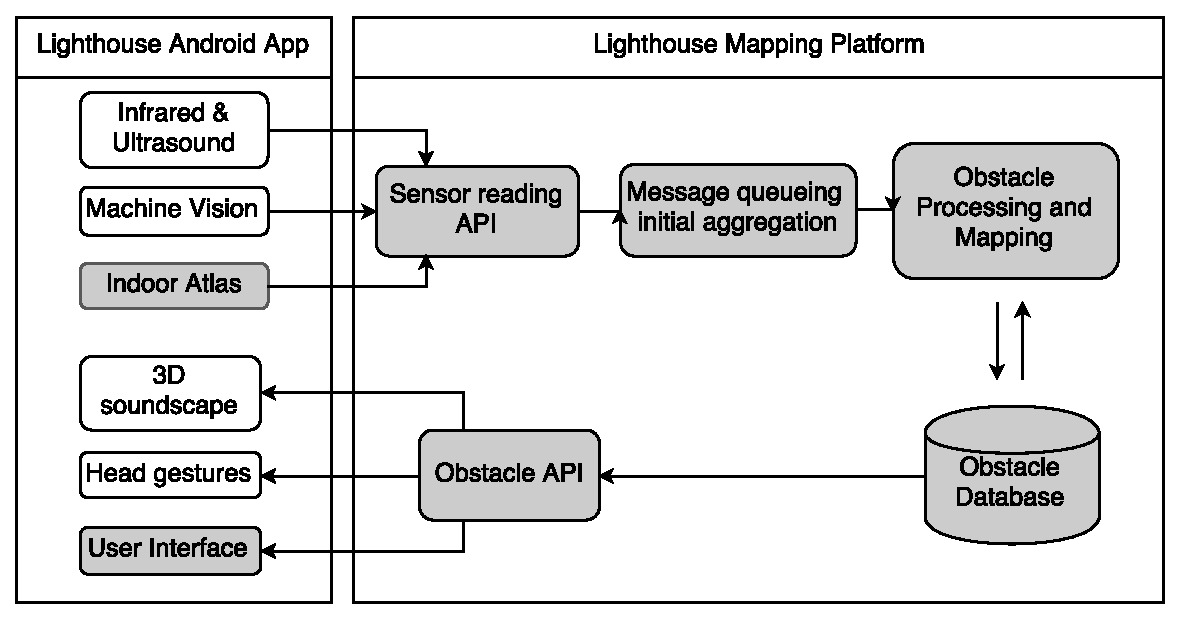
\includegraphics[width=\textwidth]{ReportDiagram.pdf}
\caption{System architecture}
\end{figure}

\subsection{Interactions}
\label{sec:interactions}
To facilitate communication between the server side and the client side the SSE team developed a portable library that handled the communication. It defines a clearly documented API for the use of the data collection and feedback applications. The library contains methods to synchronously or asynchronously send sensor readings to the data collection platform in addition to providing an API that allows the feedback applications to query the mapping platform for obstacles in an area. Each of the applications discussed in this section use these APIs to interact with the server side platform.

\subsection{Data collection and feedback}
The client side section of the project had two main jobs, one was to gather data from the sensors and relay them to the backend for further processing. The second is to give the user feedback on possible obstacles in the area and respond to commands from the user. Two of the sub components would be the responsibility of the SSE team and each of the rest would be handled by a member of the CS team. This was done as a means to decouple the work of the CS students from the work of the SSE team and remove the SSE teams dependency on the work of the CS team. By having one data collection application and one feedback application developed by the SSE team and the rest by the CS team the risk to the SSE project was therefore reduced, in the event of the CS team not being able to finish their parts of the architecture.

\subsubsection{Indoor Atlas location and obstacle listing}
The components developed by the SSE team were chosen so that a full slice of the system would be developed by the SSE team and any deliverables by the CS team would be additive. The app loads a map on to the screen of the mobile device and shows a point that represents the users location and heading.

The Indoor Atlas application uses an SDK developed by Indoor Atlas Ltd. \cite{IndoorAtlas} which uses magnetometric, accelerometer and gyroscopic sensors in a mobile device to determine a users location and heading indoors. In addition to sending the data to the server side the app also queries the server for the locations of obstacles. These obstacles are also drawn on the on-screen map.

\subsubsection{Visual obstacle detection}
The visual obstacle detection component uses a head mounted camera that takes pictures of the area in front of the user and uses a color detection algorithm to detect the floor area. Once the floor area is detected any obstacles of a different color are then be detected and their location is sent to the data collection platform.

\subsubsection{Ultrasound and Infrared}
The ultrasound and infrared component also makes measurements of the objects in front of the user and send the readings to the obstacle mapping platform.
These measurements are done by using 2 infrared sensors and ultrasound sensor to detect the distance from the user to an obstacle. The 3 sensors readings are preprocessed and filtered to mitigate the effects of temperature, velocity and other factors before being sent to the data collection platform. 

\subsubsection{3D audio training}

\subsubsection{Head gesture recognition}

\subsection{Obstacle processing and mapping}
These sensors are the minimal set of sensors decided upon for the initial iteration of the project, however the mapping platform was designed to accept any type of sensor reading. Therefore there are a few preprocessing steps between the data collection API described in section~\cite{sec:interactions} and the final obstacle processing and storage. A figure depicting the processing pipeline can be found in Appendix~\ref{app:SparkPipeline}.

\subsubsection{Data collection API}
The first point of contact in the data collection platform is the API mentioned in section~\cite{sec:interactions}. The responsibility of this component is to provide an interface for the server side that allows the data collection applications to send data to the server side platform. This is implemented by a server that listens on a UDP socket for messages in a specific JSON format. Once a message is received the message is validated and partially deserialised into a data structure and given a timestamp. The ID of the device sending the measurements is also recorded to allow the platform to correlate messages from different sensors from the same device.
%TODO: citation needed

\subsubsection{Aggregation}
\label{sec:aggregation}
After being partially deserialised the messages are filtered and split into categories. This step is designed so that the initial aggregation layer recognises the types of sensors and can map them to types that are used in the calculation of obstacles further down the pipeline. This allows for specific handling of each type of sensor in the aggregation layer while providing structured data down the line for processing. In the initial iteration there are three main data types, location, heading and distance. These sensor values are a minimum set necessary to infer the location of an obstacle based on a users location, heading and the distance to the obstacle. By abstracting the sensor values into these types the final obstacle calculations can be decoupled from the complexity of processing raw sensor readings and can be made more flexible. Once a sensor reading has been categorised it is pushed into a single message queue that is a part of a producer-consumer pattern. The producer-consumer pattern is implemented by the Apache Kafka message broker system~\cite{ApacheKafka}. Kafka provides a distributed messaging systems that allows for separation of large volumes of data into categorised streams called \"topics\". This is used by the system to sort the deserialised data structures into topics which are then processed further.

\subsubsection{Processing and Mapping}
The readings produced and pushed into the Kafka topic in the step described in section~\ref{sec:aggregation} are consumed by a consumer that is implemented in Apache Spark~\cite{ApacheSpark}. Spark is a high performance, in memory, cluster computing framework. It provides a scalable platform that is capable of efficiently computing the large amount of data that the data collection applications can output. Spark Streaming is then used on top of the Spark processing platform to process the streamed topics provided by Kafka~\cite{ApacheSparkStreaming}.

In spark the categorised and partially deserialised sensor readings are fully serialised into concrete data types and then pushed into separate streams, one for location and heading and another for distance readings. This separation is to facilitate the preprocessing and filtering done in the next step. 

Once the streams have been separated based on data type the first pass of sensor fusion is performed. There is a moving average performed over each of the streams and an aggregation done to down sample the stream to a tick rate of 100ms. This smooths out noise in the sensor signal and gives a more accurate reading for each tick, which is then fed to the mapping calculation step.

Before performing the final mapping calculation the streams are joined and aligned based on the timestamp of the sensor reading and the ID of the device that performed the reading. This is done so that the mapping calculation can draw batches of measurements from each device over a certain time interval for further calculations. The result is a stream of sensor readings that is keyed by the server tick time and grouped by device id.

The last step involves a second pass of sensor fusion that consumes batches of readings from the joined stream and passes them through a calculation that extrapolates an obstacles position from a users location, heading and the distance measured by the sensors. These obstacles are then persisted in Apache Cassandra~\cite{ApacheCassandra}.

\subsubsection{Storage and obstacle API}
Cassandra is a highly performant, distributed NoSQL database that offers the same throughput and scalability as the other Apache products discussed in previous sections. The obstacles identified by the processing pipeline are stored in a table that contains the location, confidence and ID of an obstacle.

The feedback applications can then query Cassandra for obstacles by calling the Obstacle API. This API is a REST web service written in Java that queries the table in Cassandra and exposes a simple interface to the feedback applications.


% ======================================================================================================================================================
% Given the goals the team and the client set for this project, there were several considerations to be made to make the architecture flexible and performant enough to satisfy the requirements. Having the requirement of being able to accept data from many kinds of sensors made it clear that the architecture had to be made up of a variety of strategies to homogenise the data so that it could be processed in a more abstract way. Subsequent processing can then be performed based on a fixed data model that would make it easier to develop rapidly and evaluate different processing strategies.

% As described in section~\ref{architecture} the chosen architecture uses a variety of different technologies to achieve its goal. Each component therefore had a predefined best practice in implementation. The team aimed to follow best practices when working with each technology and align their work so that each member would be able to work on each component interchangeably.

% The first concern the SSE team took on was the choice of programming language. Each of the Apache technologies supported Java, Scala and Python for development so those were the options evaluated. Java and Scala are the most common implementation languages for these technologies and provide the most comprehensive documentation and support. The team felt more comfortable with Java than Scala and the choice of using Android for the front end applications drove the decision towards using Java for the server side as well. This would help the team work together in an environment everyone was comfortable with and limit the risk posed to the project that comes with the team learning a new environment during development.





% \subsection{Data collection}
% \label{sec:dataCollection}
% The data collection aspect of the project was a major architectural concern since the data processing part of the pipeline is supposed to handle data coming from many different kinds of sensors. This part would have to be able to filter and make sense of a high volume of sensor readings and prepare them for further processing. Therefore the SSE team set up a simple, well documented, API for the data collection applications to communicate with. This decoupled the processing platform from the data collection by exposing an interface that clearly stated the data expected by the processing platform from the data collection applications.
% The initial implementation plan for this part of the architecture was to have the CS students implement each of the data collection applications, and the SSE team would implement the processing platform.
% Concern about this structure was raised by our academic stakeholders where they wanted the SSE team to decouple their work further from the CS students. This was done by having one of the data collection application implemented by the SSE team, thereby making the SSE team responsible for a full slice through the system. Any additional data collection by the CS students would therefore be additive and not essential to the success of the project.

% \subsubsection{Visual obstacle detection}
% One CS student was assigned the task of exploring the use of camera feeds to detect obstacles. The main aim of the task is to determine what specific method within the wide field of computer vision might fit best for obstacle detection. The two items that stood out were stereovision, which uses two cameras separated by a set distance, to detect the distance to each point in an image and use that to determine if there is an obstacle in the path. The second is to use colour detection to determine the floor area of a room and then mask out any parts of the image that are of a different colour, the masked out sections would then be identified as obstacles. The cameras were to be mounted on a headset and directed at an angle towards the ground in the direction the user was facing to detect obstacles in that area. The colour detection method provided the best results and was used to gather data for the mapping platform.

% \subsection{Obstacle Query API}
% To query the database an API was set up that was written in Java using the Jersey framework. The API is hosted on the same machine as Cassandra using the Tomcat web server. Upon processing by spark, a single obstacle location is stored in Cassandra with a confidence of 0 - 100. Confidence states how certain we are the obstacle would not move position with time. For example a pillar would have a higher confidence in comparison to a chair or trash can because it will hardly change its position.

% \subsection{Ultrasound and Infrared}
% Another CS student worked on an application that polled cheap off-the-shelf infrared and ultrasound range finding sensors. These sensors would, like the computer vision cameras, make measurements of the objects in front of the user and send the readings to the obstacle mapping platform.

% \subsection{Feedback}
% After Processing, the obstacle data will be stored in Cassandra database. Based on the Requirement mentioned in Section 3.4, we implement the feedback part to show the user the surroundings by querying the stored obstacle data. When to query the nearby obstacles in the database, we set the query based on the user‘s location data which consists of latitude, longitude and radius. In an actual situation where our platform is used for, we show the obstacles nearby instead of all the obstacles detected and stored. For this reason, we set radius which allows the platform give user feedback within an exact area. We show the obstacle both in a scrollable list and on a visual map.


%Kafka is a distributed publish subscribe messaging service designed specifically to be fast and handle large volume of data inflow coming from various sources. Kafka is fault tolerant as it is inherently distributed over a cluster computers so if one broker fails, the other live brokers will complement the node. Kafka achieves fault tolerance with the help of zookeeper which is a separate Apache tool for configuration and synchronisation of nodes in a distributed system. A leader in a Kafka broker is responsible for read/write operations in a partition and only one leader can exist for every partition. If a leader dies in the cluster, zookeeper is responsible for managing change in leadership to an existing slave broker. Furthermore Kafka seamlessly integrates with Spark for high speed data processing. 

%\subsection{Processing}
%With Apache Kafka working as a producer for the producer/consumer pattern and Apache Spark working as the consumer the team managed to handle the level of throughput needed for the purposes of the project.
%Spark consumes streams of sensor readings coming from Kafka in the distributed way, performs the processing on the data and stores the result into database.




% \subsection{Aggregation}  % TODO: find a good name for this
% The API mentioned in Section~\ref{dataCollection} was the only contact point for the data collection applications. The component needed to be designed and implemented to handle large quantities of incoming readings, from many different sources, and efficiently buffer and pass them to the processing component. The aggregation component would group together readings and post them to the processing component in a producer/consumer pattern. To manage this the SSE team evaluated several message broker systems for the job, Apache Kafka, Azure EventHub and RabbitMQ. The criteria used was threefold, one was the applicability of the technology to the producer/consumer pattern, their cost and their ease of integration with the technology used in the processing component. Azure EventHub was considered as a robust and scalable possibility but was discarded because of the cost associated with running it for the duration of the project, see Appendix~\ref{ArchitectureCost}. RabbitMQ and Apache Kafka both fit well with the architecture and patterns the team had in mind but ultimately Apache Kafka was chosen because of it's ease of integration with Apache Spark.

% Kafka is a distributed publish subscribe messaging service designed specifically to be fast and handle large volume of data inflow coming from various sources. Kafka is fault tolerant as it is inherently distributed over a cluster computers so if one broker fails, the other live brokers will complemenent the node. Kafka achieves fault tolerance with the help of zookeeper which is a seperate Apache tool for configuration and synchronisation of nodes in a distributed system. A leader in a kafka broker is resposnible for read/write operations in a partition and only one leader can exist for every partition. If a leader dies in the cluster, zookeeper is responisble for managing change in leadership to an existing slave broker. Furthermore Kafka seamlessly integrates with Spark for high speed data processing. 

% \subsection{Kafka Producer Listener}
% At the listening end we would essentially do a partial deserialisation of the data packet into a JSON object to obtain the topics from each packet. Afterwards the JSON object is published into the kafka cluster.

% \subsubsection{Kafka}
% The main quality requirement for the UDP socket server for the Kafka producer was the throughput. Therefore load tests were the main focus in the testing strategy for this component. Since the component uses UDP the metrics gathered were to measure number of packets processed, number of packets dropped and the processing speed of each packet from the socket and into the message queue. The team considered using unit testing and integration tests to evaluate this component but the work involved in mocking out dependencies was not the most efficient use of time. The Kafka producer should contain as little logic as possible and therefore unit tests would be of little value. Integration tests on this component would be run when testing the integration with the Spark processing component.






% \subsection{Processing}
% With Apacha Kafka working as a producer for the producer/consumer pattern and Apache Spark working as the consumer the team managed to handle the level of throughput needed for the purposes of the project.
% Spark consumes streams of sensor readings coming from Kafka in the distributed way, performs the processing on the data and stores the result into database.
% %Describe
% \subsection{Spark}
% After Kafka has indexed, filtered and sorted the sensor readings into topics, Spark takes over and pushes the sensors reading streams through several mappings, calculations and reductions to form a processing pipeline that results in the identification of the obstacles around. In the Figure \ref{fig:Spark pipeline} the processing pipeline is described. From the pipeline it can be seen that Spark consumes data from Kafka as stream of data. Afterwards, the stream is separated into location and distance stream. Then the streams are separately processed by using moving average algorithm. After that the streams are joined into one stream and then association of the distance and location data is performed. This is done in order to be able to make the calculation regarding the location of the identified obstacle. The last step in the processing is identifying the obstacles.

% \subsection{Processes}
% The SSE team managed their work by relying on the Scrum methodology. Work was organised into 2 week sprints and standup meetings were scheduled for communication and status updates. Mondays were set up as meeting days to synchronise with stakeholders, academic supervisors and our client. Standup meetings were held the following Tuesday which was used to re-organise and adapt the work schedule over the week to the most recent project vision of our client. Fridays were used to write reports and inform our stakeholders of the progress made. The team would hand in a weekly report and send demonstration material to the client to show progress and receive feedback.
%\subsection{Android app and Jar file}
% A socket on our VPS will be listening indefinitely on a particular port for incoming data from our various sensing hardware. Each sensor or combination of sensors will measure data, do some preprocessing before sending data across to our VPS over a UDP connection. For instance one of the CS students would send three distance estimates based on the measurements collected from 2 ultrasound and 1 infrared sensor. To simplify the development process for each application the SSE team decided to provide each application with a library that would perform the data sending and obstacle querying. Therefore, reducing the code duplication over the android applications.





% \subsection{Storage and API}
% The obstacles identified by the Spark stream processing are finally persisted in a database for further processing and use by the feedback applications. The database used for persistence needed to fulfil several requirements to fit the project, scalability with increased load, flexibility of schema and cost.
% The scalability can be solved by most distributed databases but the flexibility of schema and cost are more difficult to work around.
% The first step in the choice of database technology was to decide on a SQL or NoSQL database, where NoSQL provided the flexibility needed. After NoSQL was selected the next question was whether to go for a document storage or column storage database. Both provide a flexible schema data persistence but the data modelling needed for each is quite a bit different. After these deliberations there were 3 possibilities explored, Apache Cassandra, Azure DocumentDB and MongoDB.  Here again the cost of running an Azure product is prohibitive to an academic prototype project, in addition to that the documentation and troubleshooting resources of the open source technologies is far better than the ones available for Azure. Apache Cassandra and MongoDB both seemed to fit well with the needs of the architecture, both are easily integrated with Spark and both have more than adequate documentation. The deciding factor in choosing between the two was the fact that Cassandra is an Apache distributed system that inherently works with Zookeeper in the same way that Spark and Kafka do. This meant that the time and effort in setup and maintenance would be lessened since all these technologies run in the same managed distributed environment.

% \subsection{Cassandra}
% The data modelling for Cassandra was fairly simple, the number of data points needed to persist an obstacle were few and clear. After setting up the Cassandra server the data model was set up through CQL and drivers with Java set up for testing and querying.


% % TODO: make a good argument for how we managed RISK



% \section{Implementation}

% \subsection{Android app and Jar file}
% A socket on our VPS will be listening indefinitely on a particular port for incoming data from our various sensing hardware. Each sensor or combination of sensors will measure data, do some preprocessing before sending data across to our VPS over a UDP connection. For instance one of the CS students would send three distance estimates based on the measurements collected from 2 ultrasound and 1 infrared sensor.


\section{Evaluation}
Given the nature of the project the main success criteria is if the system can accurately determine the location of an obstacle in space based on the sensor data given. The evaluation of this fact was done by doing experiments with the actual sensor hardware, extracting the noise level, accuracy and other quality metrics and then generating sensor output based on those metrics. This generation of test data allowed us to evaluate the accuracy of our system in a controlled environment. We evaluated the robustness of our processing methods by increasing the noise in the generated sensor signal in addition to controlling the rate of data sent to the system. The throughput of the system was also evaluated by sending large amounts of sensor readings at a time and measuring response time, packet loss and transmission delay.

\section{Testing strategy}
To test if the quality of the Lighthouse project meets the standard of the client, testing procedures were made via experience. Since different components of the architecture have different feature to test, unit, load and integration tests were implemented separately.

\subsection{Unit testing}
Unit testing is a kind of software process where small parts of the application are tested individually and independently to check if they are in proper operation. (add citation) In Lighthouse project, unit testing was used for Obstacle API which had several logic components. Each logic was tested with actual data independently to assure each part run the correct logic.

\subsection{Load testing}
Load testing is a process of putting demand and checking response, which will be undertaken in both normal conditions and overload conditions. (add citation) For the components which deal with input and output stream, load testing is a useful testing strategy.
First, the Kafka component which managed the message queue in the project was tested with different amount data simulated by code. Then, load testing will be performed on Spark processing throughput, since the entire processing pipeline needs to be checked for bottlenecks which will affect the response time of the whole project. Also, load testing is used to test the Obstacle API to make sure the API stands up to a minimum level of pressure expected in our quality requirements.

\subsection{Integration testing}
Integration testing is a test strategy where individual parts of the project are combined and testing together as a group. Integration testing can show how the whole project works via testing the interfaces between components, interactions to different parts of the system. 
Since the dependency of the processing component on the Spark environment creates real problems to unit testing, integration tests were found to be sufficient to assure the team that the processing is producing the correct results when the unit testing is hard to perform.
Integration testing will be carried out after all the tests mentioned above to check if the processing is producing the correct output.
\subsection{Other testing}
Besides all the testing methods above, other tests were also used in this project. For the data collection part, accuracy and response time are the most important feature to be tested. The latency will be tested by recording the time when sending the data and the time when getting the response. Overall 20 testing will be taken, and the average result is the latency. To test the accuracy, the actual accuracy will be measured by calculating the distance between the actual user location and the Indoor Atlas result.


\subsection{Tools and Data generation}
The data was generated through a simulation script written in Python. The simulation was set up by specifying an agent, some obstacles and a set of sensors. The agent and obstacles would have a location in space and the agent had a maximum velocity, rotation speed and other movement parameters. The simulation would then be configured by laying out a path for the agent to move through while the sensors were polled to check if they would detect an obstacle. The simulation allowed for noise to be added to the sensor readings that would give a more realistic way of processing sensor data that will inherently contain error and noise.

\subsection{Performance and Scalability}
After implementing the processing pipeline the first performance test performed was to evaluate the throughput and packet loss. This was done by sending progressively larger numbers of simulated sensor readings to the pipeline and measure how it handled the load.

\begin{center}
\begin{tabularx}{\textwidth}{| X | X | X | X |} 
\hline
\# Readings & Transmission time & \# Readings/Second & Packet Loss \% \\
\hline
7400 & 2.220366535 & 3332.783071 & 1.135135135 \\
\hline
74000 & 15.81466027 & 4678.380612 & 0.7731087894 \\
\hline
740000 & 119.9508543 & 5738.18339 & 5.847595525 \\
\hline
\end{tabularx}
\label{tab:performance}
\end{center}

The results shown in table~\ref{tab:performance} show that the pipeline handled loads far beyond what was stipulated in the quality requirements, the packet loss is within acceptable limits (2\%) for over 100000 readings and the throughput was an order of magnitude higher than the goal. The quality requirements needed the pipeline to handle 100 readings per second but the load testing showed that the pipeline could handle over 5000 messages before it started to experience deteriorating performance.

% \begin{figure}
% \centering
% \subfigure[Figure 1] {
%   \label{fig:sub1}
%   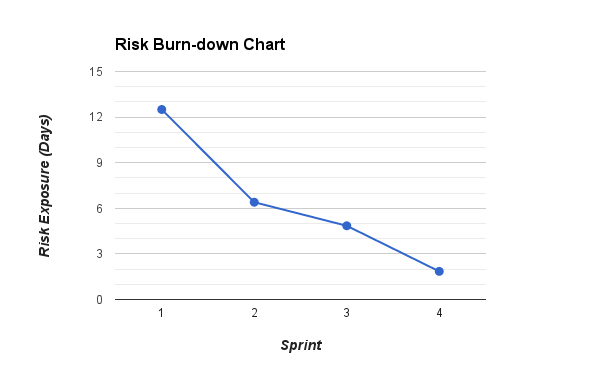
\includegraphics[width=.3\linewidth]{burndown-chart}
% }
% \subfigure[Figure 2] {
%   \label{fig:sub1}
%   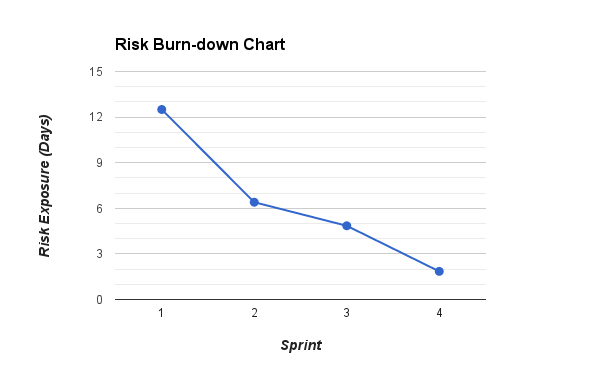
\includegraphics[width=.3\linewidth]{burndown-chart}
% }
% \subfigure[Figure 3] {
%   \label{fig:sub1}
%   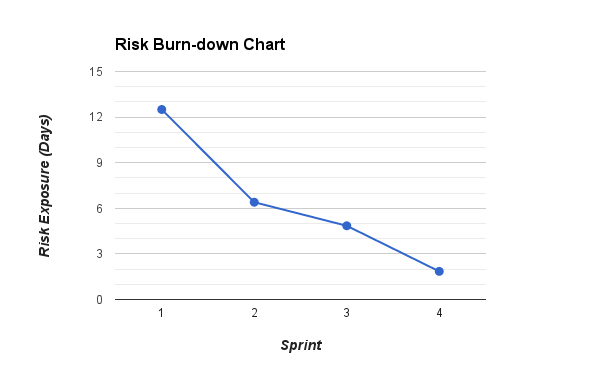
\includegraphics[width=.3\linewidth]{burndown-chart}
% }
% \caption{A figure with two subfigures}
% \label{fig:test}

% \subfigure[Figure 4] {
%   \label{fig:sub1}
%   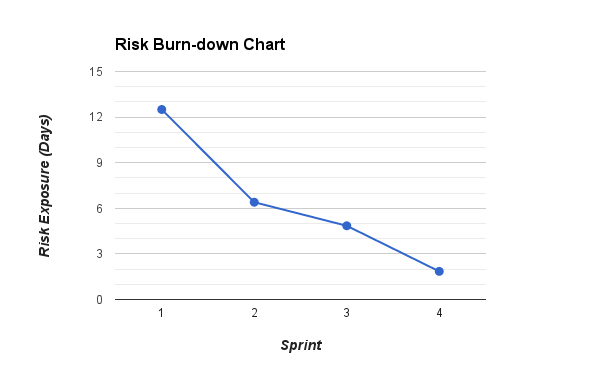
\includegraphics[width=.3\linewidth]{burndown-chart}
% }
% \subfigure[Figure 5] {
%   \label{fig:sub1}
%   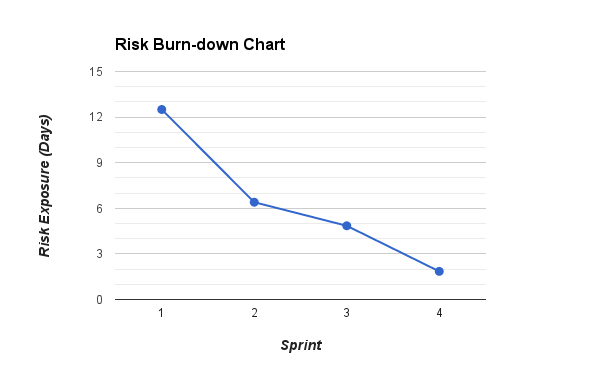
\includegraphics[width=.3\linewidth]{burndown-chart}
% }
% \subfigure[Figure 6] {
%   \label{fig:sub1}
%   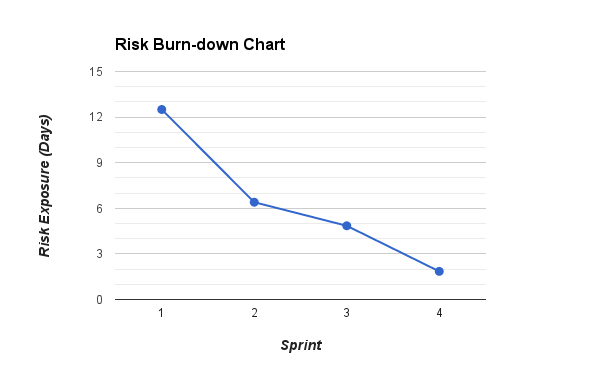
\includegraphics[width=.3\linewidth]{burndown-chart}
% }
% \caption{A figure with two subfigures}
% \label{fig:test}
% \end{figure}

\subsection{Detection accuracy}
Describe the testing scenario, the simulator and show diagrams that compare both.


\subsection{Acceptance}
%TODO: Talk about the cs students evaluation?

\subsection{Android application}
We decided to program in an android environment because the team is more familiar with programming in Java as opposed to C\# and Objective C/Swift for Windows phone and IOS respectively. Moreover the team decided to use Java in building the components of our overall architecture, so it will be a good fit for the team to keep everything Java. Additionally the team helped with dealing with bugs, syntax and programming logic because we all focused on leveraging one programming language. This helped the team work together in an environment everyone was comfortable with and limit the risk posed to the project that comes with the team learning a new environment during development.

\section{Challenges and Lessons Learnt}
\subsection{Initially Proposed System}
\label{sec:Prelim}
%TODO: citation 
The initial plan for this project was to make use of device developed by students in the Electrical Engineering department. The hardware consists of an armband that can detect ultrasonic frequencies. Those frequencies are emitted by at least 3 beacons in strategically predefined locations in the room. The armband, in conjunction with a computer and an Android device, then triangulates the position of the armband in space.
The former use cases to be explored focused on detecting gestures and possible indoor location possibilities. However, soon after the project was presented to the team, the hardware was found to have several limitations. The team found that the location accuracy was considerably less than what was initially described. The initial description of the hardware stated that the location accuracy was sub-centimetre, which is the theoretical minimum, but the functional accuracy was between 10 and 50 centimetres. This eliminates the gesture use case since more precision is needed to get accurate gesture recognition.
%TODO: citation
Furthermore, the hardware can only function if 3 beacons are within a 130\degree cone in front of the receiver. This severely limits the practicality of the device for indoor location since a wearable piece of hardware is usually blocked by the wearer's body in addition to any obstacle in the environment such as static or movable objects.
%TODO: citation
Therefore the high probability of getting unacceptable performance out of the hardware platform was found to cause too much risk to the project and the team mitigated that risk by pivoting the focus of the project to a different topic.

\subsection{Testing with Real Data}
Despite creation of a program which simulates an user who moves in an environment full of obstacles, we could be never sure that our system fulfil the requirements. It is because the real data was expected to be provided by the CS students and it could differ from the data provided by the simulator. The challenge was that the CS student could provide real data only during the last few week of the project which gave us little time to test our platform with real data. 

\subsection{Memory Shortage}
Initially we rented a private server with only 2GB of main memory to run Oracle Java, Scala, Jenkins, Spark, Kafka, Zookeeper, Tomcat and Cassandra. Before we rented the server we had little prior knowledge our tools are memory intensive hence the server froze intermittently due to a shortage of memory. In addition to the server freezing, some of our tools could not start up for example Kafka and Zookeeper displayed error due incapacity of the Java virtual machine to allocate sufficient memory required to start up both tools. 

To resolve our memory troubles we upgraded our subscription to a machine with 6GB of main memory and 25GB of secondary memory. Furthermore we allocated swap space of 6GB deal with any unforeseeable eventuality. Lastly we set the machine to depend highly on main memory in order to keep I/O operations as fast as possible.

This situation had been avoidable if a thorough evaluation of the hardware requirements of all the technologies had been made in the early weeks of development.

\subsection{Shared communication library}
As described above a library was provided to the CS students which let them interact with our platform. Initially, we decided to implement this library on a desktop computer using Java 8. However, when we tried to use the library to send data to our platform we realised that android has several limitations on how it performs networking tasks. Specifically, it would not let to send data over socket on the main thread. Therefore, we had to re-implement the library to be compatible with android devices. The effect of this problem was slightly mitigated by the fact the SSE team developed one of the data collection applications, this meant that the testing of the library could be done fully by the SSE team without having to send it to the CS students for testing.

\subsection{Java over Scala for Spark}
As described above it was decided to use Java as a programming language for Spark processing. Making this decision led us to several challenges which we couldn't know beforehand. First, despite that there was plenty of Java code documentation we still spent a lot of time on implementing the required features. That is due to the fact that the official Java code was not working anymore with the latest Spark version because of methods deprecation. Therefore, we were forced to learn the technology more deeply in order to workaround these problem. 

From the experience with Spark programming we have learned that sometimes it is better to learn a new language for which the technology was initially implemented instead of picking an already familiar language in order to program on the new technology. In addition, the code would be much cleaner if we had used Scala instead of Java.

\subsection{Combining Data Streams}
Another challenge, on top of absence of up-to-date documentation, was understanding how Spark is processing data and how to write code for it. Initially the sensor data processing was written in standard Java 8. We encountered several problems when tried to integrate the code into Spark since it uses different concept of data, where data stream contains batches of sensor data. First, Spark didn't let us to work with sensor data in different batches as we expected. Therefore, we had to completely change the processing approach, which also took us time.

The experience was helpful to understand that implementation of features should be right away done for the technology which is going to be used.

\subsection{Cassandra Data Modelling}

\subsection{Completing Tasks in Sprints}\textcolor{orange}{debatable though!. Was going to say something about having too many tasks in a sprint and ending up having to carry over tasks to the next sprint and etc.}

\section{Life cycle and Future Work}
\subsection{Current state}
The Lighthouse project now can process data from two kinds of sensors, location and rangefinding sensirs, and achieves the aim of detecting obstacles through the use of them. The project reaches the goal of using low-cost and off-the-shelf sensors. Currently, the magnetic sensor in the android device, camera, Inferred and Ultrasound sensors works together to collect data from the indoor environment and send all the information collected to data processing component by implementing the API created by SSE team. After the processing, feedback will be shown to users in map and 3D sound. The two most important factor of performance are latency and accuracy. In our testing mentioned above, the quality of the project can fulfill the requirement of indoor real-time obstacle detection.(need to add some testing result)

\subsection{Future work}

\subsubsection{Sensor fusion}

\subsubsection{NoSQL to MySQL}

\subsection{Maintenance and Scaling}
% TODO: Enumerate limitation of the product
% TODO: Describe how we can go from prototype to a running system
In the future, when the project needs to be expanded with other types of sensors, this platform can still provide the interface for communication between device and processing component. 
Although this product can fulfil the client's requirements, it has huge performance disparity with a real industry product. Since budget and experience are limited, the capability of the project is not sufficient to support thousands of simultaneous user queries at the moment.

This project can be migrated to Azure which is a Microsoft product and can provide global coverage and high availability and stability. The components of the project need to be rewritten in C\# and Azure analog technologies. Please refer to Appendix~\cite{app:MigrationPlan} for a detailed description of a possible migration strategy.


\section{Conclusion}

% TODO: identify the topic takeaway messages.
% takeaway messages describe how we one could do things differently.
% not in context of the project but rather in the context of the domain. 

% Appendix
\appendix
\section*{APPENDIX} \label{Appendix}
\setcounter{section}{1}

\appendixhead{ZHOU}

% Acknowledgments
\begin{acks}
\end{acks}  

% Bibliography
\bibliographystyle{ACM-Reference-Format-Journals}
\bibliography{GroupReport-bibfile}

% History dates
%\received{February 2007}{March 2009}{June 2009}

% Electronic Appendix
\elecappendix

\medskip

\section{Migration plan}
\label{app:MigrationPlan}
\section{This is an example of Appendix section head}

\pagebreak
\section{Spark Pipeline Figure}
\label{app:SparkPipeline}
\begin{figure}[!ht]
\label{fig:SparkPipeline}
\centering
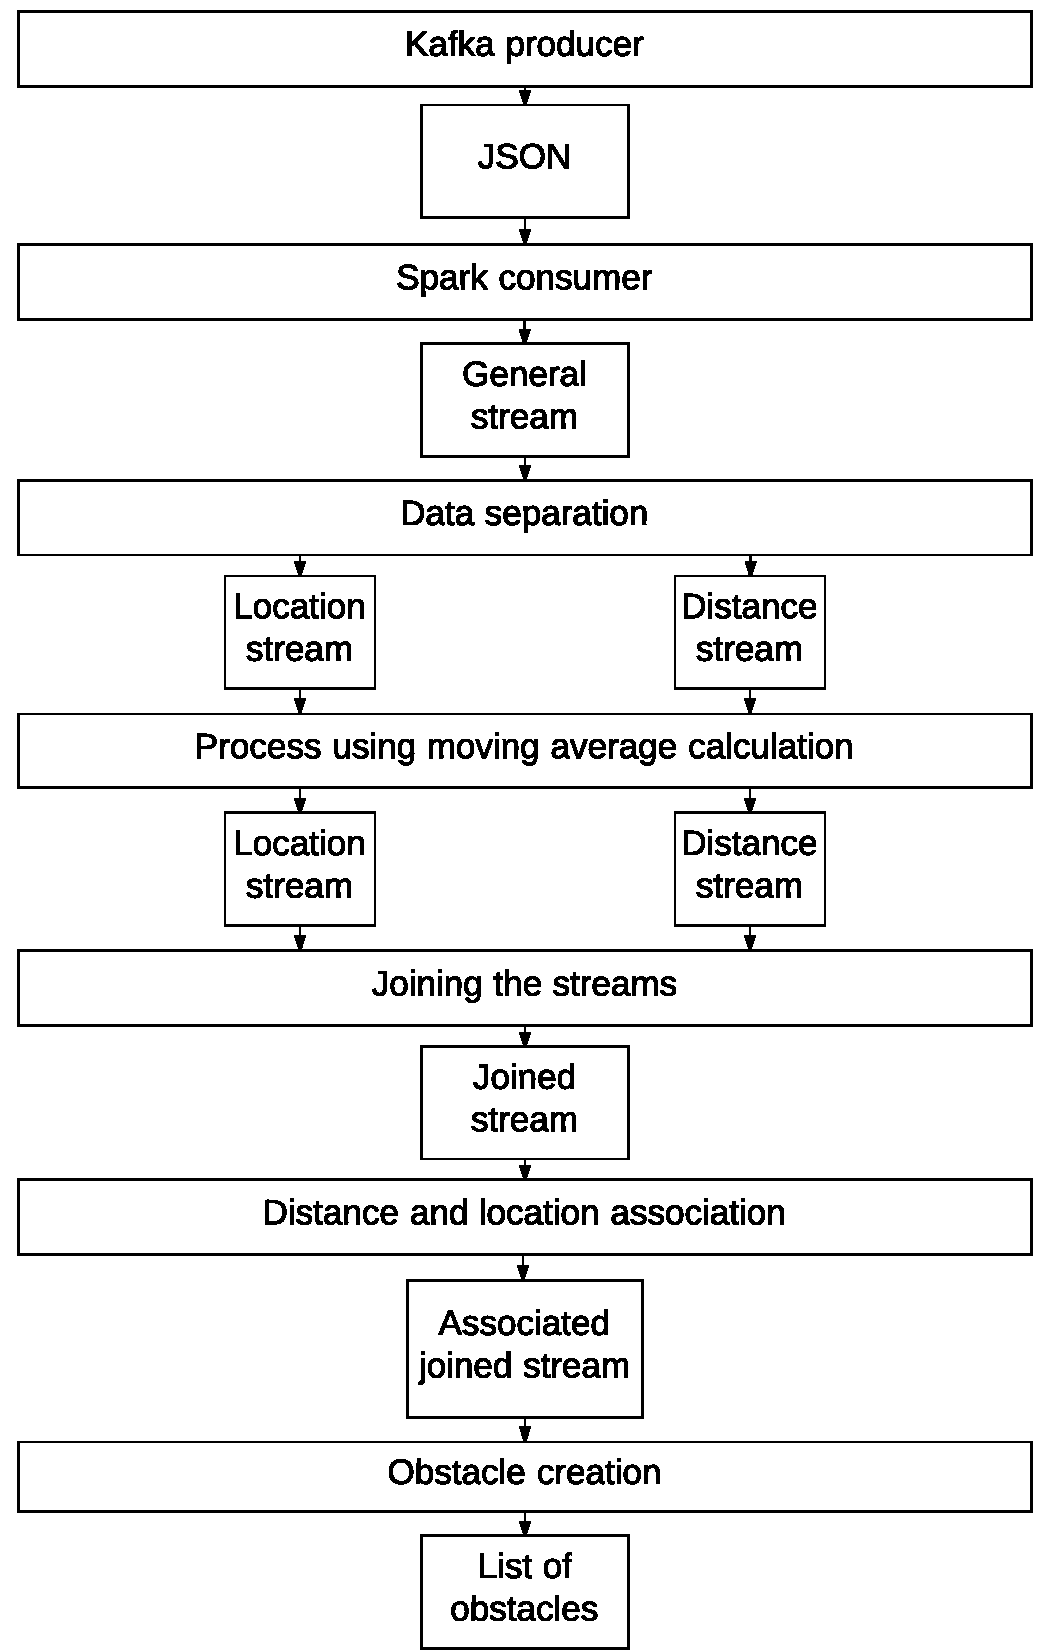
\includegraphics[width=0.8\textwidth]{SparkPipeline.pdf}
\caption{Spark processing pipeline}
\end{figure}
\clearpage
\pagebreak
\section{Architecture cost analysis}
\label{ArchitectureCost}

\end{document}



